Mục tiêu của bước này là tạo ra một tập dữ liệu đủ lớn, phản ánh toàn diện các trạng thái biến động của thị trường, đặc biệt là các cú sốc giảm giá đồng loạt. Quy trình mô phỏng được thực hiện như sau:
\begin{itemize}
    \item Khởi tạo kịch bản từ hàm Copula: Thuật toán sinh ra 10.000 vector quan sát đồng nhất từ hàm t-Student Copula với bậc tự do $df=4$. Ma trận này chứa đựng trọn vẹn đặc tính đuôi nặng và cấu trúc tương quan phi tuyến giữa 4 cổ phiếu công nghệ.
    \item Khôi phục phân phối biên bằng ECDF: Để đảm bảo các kịch bản lợi suất không bị ép vào khuôn khổ phân phối chuẩn, nghiên cứu sử dụng hàm phân phối tích lũy thực nghiệm (Empirical CDF - ECDF). Các giá trị đồng nhất được ánh xạ ngược ($F^{-1}$) về thang đo tỷ suất sinh lợi thực nghiệm, giúp giữ nguyên vẹn độ lệch và độ nhọn của dữ liệu thực nghiệm.
\end{itemize}

\begin{figure}[H]
    \centering
    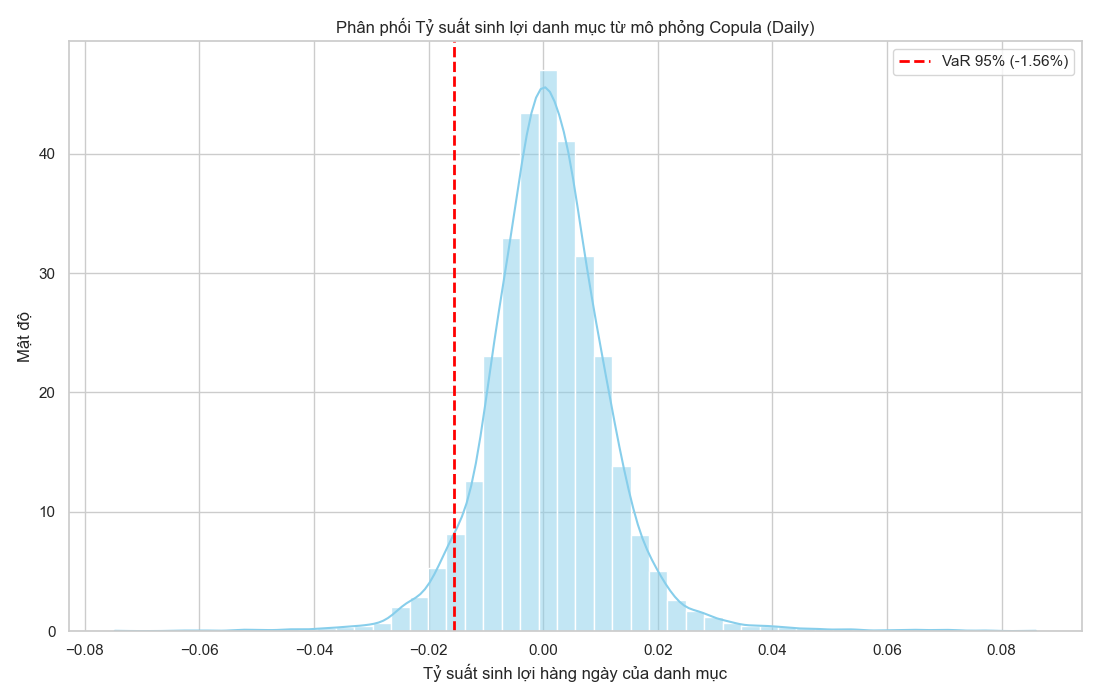
\includegraphics[width=0.85\textwidth]{copula_monte_carlo_daily_var.png}
    \caption{Phân phối tỷ suất sinh lợi hàng ngày của danh mục từ mô phỏng Copula}
    \label{fig:daily_return_dist}
\end{figure}

\begin{flushleft}
Quan sát Hình \ref{fig:daily_return_dist}, phân phối lợi suất hàng ngày thể hiện rõ đặc tính nặng đuôi. Đối với danh mục phân bổ đều ban đầu, ngưỡng rủi ro VaR 95\% được xác định ở mức -1.56\%, nghĩa là trong điều kiện thị trường bình thường, xác suất danh mục giảm sâu hơn mức này chỉ giới hạn ở 5\%. Đây là cơ sở dữ liệu nền tảng để tiến hành tối ưu hóa CVaR ở bước tiếp theo.
\end{flushleft}